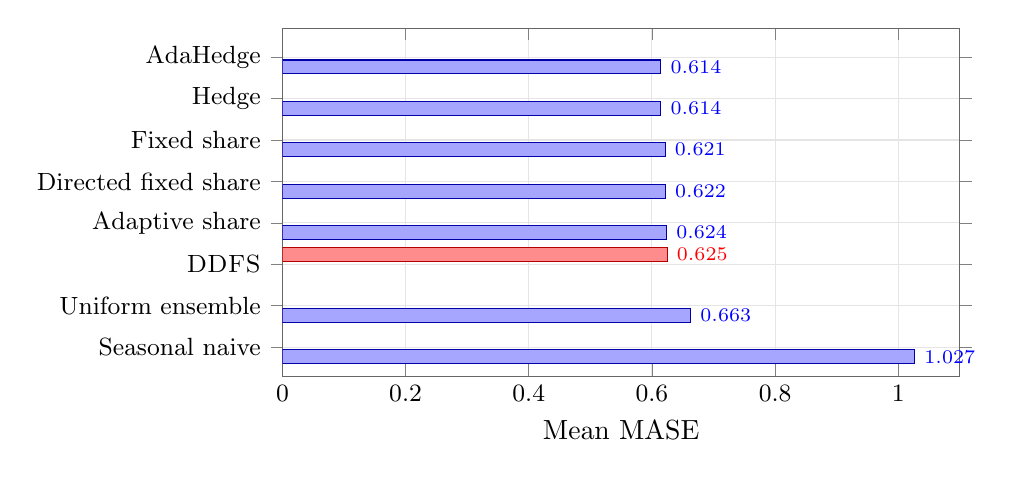
\begin{tikzpicture}
\begin{axis}[
  xbar,
  width=0.84\linewidth,
  height=6.0cm,
  xmin=0,
  xmax=1.10,
  xlabel={Mean MASE},
  ytick={0,1,2,3,4,5,6,7},
  yticklabels={Seasonal naive,Uniform ensemble,\textsc{DDFS},Adaptive share,Directed fixed share,Fixed share,Hedge,AdaHedge},
  yticklabel style={font=\small},
  xticklabel style={font=\small},
  bar width=5pt,
  nodes near coords,
  nodes near coords style={font=\scriptsize,/pgf/number format/fixed,/pgf/number format/precision=3},
  grid=major,
  grid style={gray!20},
  axis line style={black!60},
]
\addplot+[draw=blue!65!black,fill=blue!35] coordinates {(0.614409082,7) (0.614464765,6) (0.621467303,5) (0.621915883,4) (0.623638880,3) (0.662893327,1) (1.026539640,0)};
\addplot+[draw=red!70!black,fill=red!45] coordinates {(0.624662497,2)};
\end{axis}
\end{tikzpicture}
